%%%%%%%%%% !TEX program = xelatex %%%%%%%%%%
% !TEX program = xelatex
% !Mode:: "TeX:UTF-8"
% \def\usewhat{dvipdfmx}                            % 定义编译方式 dvipdfmx 或者 pdflatex ,默认为 dvipdfmx
% 方式编译,如果需要修改,只需改变花括号中的内容即可。
\documentclass[xcolor=table]{beamer}% xcolor宏包的\rowcolor命令需要给宏包加table选项
%%%%%%%%%% 幻灯片导言区 %%%%%%%%%%%
\usepackage[UTF8,noindent]{ctex}% ctex只引入必要的中文,ctexcap还会翻译图表等环境名称
%%%%%%%%%% 加入必须的宏包(如自己有特殊宏包需要可以加到这里) %%%%%%%%%%%
\usepackage{color}
\usepackage{graphicx}
\usepackage{subfigure}
\usepackage{caption}
\usepackage{lipsum}
\usepackage{array}
\usepackage{listings}% 使用listings包
\usepackage{multirow}% 使用multirow宏包,使得表格可以合并多个row格
\usepackage{booktabs}% 表格,横的粗线;\specialrule{1pt}{0pt}{0pt}
\usepackage{multicol}% 多栏宏包
\usepackage{wasysym}% 符号支持宏包
\usepackage{amsthm}
%%%%%%%%%% 加入Times New Roman字体的支持 %%%%%%%%%%%
\usepackage{amsmath}
\usepackage{times}
\usepackage{mathptmx}
\usepackage{colortbl}
%%%%%%%%%% 书签中文支持 %%%%%%%%%%%
\usepackage{hyperref}% 设置书签
%\hypersetup{bookmarks, unicode}% 书签编码格式
%%%%%%%%%% 参考文献支持 %%%%%%%%%%%
\usepackage[backend=bibtex,sorting=none]{biblatex}% 参考文献
\setbeamertemplate{bibliography item}{% 根据Bibtex中的Entrytype类型来选择图标
	\ifboolexpr{ test {\ifentrytype{book}} or test {\ifentrytype{mvbook}}
		or test {\ifentrytype{collection}} or test {\ifentrytype{mvcollection}}
		or test {\ifentrytype{reference}} or test {\ifentrytype{mvreference}} }
	{\setbeamertemplate{bibliography item}[book]}
	{\ifentrytype{online}
		{\setbeamertemplate{bibliography item}[online]}
		{\setbeamertemplate{bibliography item}[article]}}%
	\usebeamertemplate{bibliography item}}

\defbibenvironment{bibliography}
{\list{}
	{\settowidth{\labelwidth}{\usebeamertemplate{bibliography item}}%
		\setlength{\leftmargin}{\labelwidth}%
		\setlength{\labelsep}{\biblabelsep}%
		\addtolength{\leftmargin}{\labelsep}%
		\setlength{\itemsep}{\bibitemsep}%
		\setlength{\parsep}{\bibparsep}}}
{\endlist}
{\item}
\addbibresource{slide.bib}% 参考文献数据库文件,放置到同级目录,名称是bib文件名,可以修改
%%%%%%%%%% 去掉子图标号 %%%%%%%%%%%
\makeatletter
\renewcommand{\@thesubfigure}{\hskip\subfiglabelskip}
\let\@@magyar@captionfix\relax
\makeatother
%%%%%%%%%% 设置自定义颜色 %%%%%%%%%%%
\definecolor{hnuBlue}{rgb}{0.2,0.2,0.6}% PPT标题颜色
\definecolor{tableHead}{rgb}{0.266,0.447,0.780}% 定义表格标题栏颜色
\definecolor{tableDeep}{rgb}{0.851,0.886,0.953}% 定义表格中的浅蓝色,浅色为默认白色
\setbeamercolor{title}{fg=black}% 设置首页标题字体颜色
\setbeamercolor{section in toc}{fg=black}% 设置目录中显示字体颜色
\setbeamertemplate{section in toc shaded}[default][50]% 设置目录中显示浅色字体颜色
\setbeamertemplate{frametitle}[default][left]% 设置每帧PPT标题位置(偏左显示)
\setbeamercolor{frametitle}{fg=hnuBlue}% 设置每帧PPT大标题颜色
\setbeamercolor{framesubtitle}{fg=black}% 设置每帧PPT小标题颜色
\setbeamercolor{navigation symbols}{ }% 取消导航条
\setbeamertemplate{sidebar right}{ }
%%%%%%%%%% 设置自定义页脚 %%%%%%%%%%%
\setbeamertemplate{footline}{% 设置页脚显示,姓名、题目和日期都已经注释掉,需要可以自行开启
\leavevmode%
\hbox{%
% 左侧1/3部分显示姓名信息
\begin{beamercolorbox}[wd=.333333\paperwidth,ht=2.25ex,dp=1ex,center]{author in head/foot}% 设置页脚长度、高度、深度等
\usebeamerfont{author in head/foot}
%\insertshortauthor% 插入姓名
\end{beamercolorbox}
% 中间1/3部分显示标题信息
\begin{beamercolorbox}[wd=.333333\paperwidth,ht=2.25ex,dp=1ex,center]{title in head/foot}  % 设置页脚长度、高度、深度等
\usebeamerfont{title in head/foot}
%\insertshorttitle% 插入题目
\end{beamercolorbox}
% 右侧1/3部分显示时间页码信息
\begin{beamercolorbox}[wd=.333333\paperwidth,ht=2.25ex,dp=3ex,right]{date in head/foot}   % 设置页脚长度、高度、深度等
\usebeamerfont{date in head/foot}
%\insertshortdate{}\hspace*{2em} % 插入日期
\insertframenumber{} / \inserttotalframenumber\hspace*{4ex}% 插入页码(显示格式:当前页/总页码)
\end{beamercolorbox}
}
\vskip0pt%
}
%%%%%%%%%% 字体及字号定义 %%%%%%%%%%%
\usefonttheme{serif}  % 设置衬线字体
\newcommand{\song}{\CJKfamily{zhsong}}                       % 宋体
\newcommand{\fs}{\CJKfamily{zhfs}}                           % 仿宋体
\newcommand{\kai}{\CJKfamily{zhkai}}                         % 楷体
\newcommand{\hei}{\CJKfamily{zhhei}}                         % 黑体
\newcommand{\li}{\CJKfamily{zhli}}                           % 隶书
\newcommand{\fssishi}{\fontsize{40pt}{40pt}\selectfont}    % 40pt, 单倍行距
\newcommand{\fssanliu}{\fontsize{36pt}{36pt}\selectfont}   % 36pt, 单倍行距
\newcommand{\fssaner}{\fontsize{32pt}{32pt}\selectfont}    % 32pt, 单倍行距
\newcommand{\fserba}{\fontsize{28pt}{28pt}\selectfont}     % 28pt, 单倍行距
\newcommand{\yihao}{\fontsize{26pt}{26pt}\selectfont}      % 一号, 单倍行距
\newcommand{\xiaoyi}{\fontsize{24pt}{24pt}\selectfont}     % 小一, 单倍行距
\newcommand{\erhao}{\fontsize{22pt}{22pt}\selectfont}      % 二号, 单倍行距
\newcommand{\xiaoer}{\fontsize{18pt}{18pt}\selectfont}     % 小二, 单倍行距
\newcommand{\sanhao}{\fontsize{16pt}{16pt}\selectfont}     % 三号, 单倍行距
\newcommand{\xiaosan}{\fontsize{15pt}{15pt}\selectfont}    % 小三, 单倍行距
\newcommand{\sihao}{\fontsize{14pt}{14pt}\selectfont}      % 四号, 单倍行距
\newcommand{\xiaosi}{\fontsize{12.5pt}{12.5pt}\selectfont} % 小四, 单倍行距
\newcommand{\wuhao}{\fontsize{10.5pt}{10.5pt}\selectfont}  % 五号, 单倍行距
\newcommand{\xiaowu}{\fontsize{9pt}{9pt}\selectfont}       % 小五, 单倍行距
\newcommand{\liuhao}{\fontsize{8pt}{8pt}\selectfont}       % 小五, 单倍行距
\newcommand{\bz}{\color{white}}                            % 白色字
%%%%%%%%%% 设置局部字体和颜色 %%%%%%%%%%
\usepackage[labelfont=bf,textfont={bf}]{caption}% 设置caption样式
\setbeamerfont{caption}{size=\xiaosi}% 设置caption字号为小四
\setbeamerfont{date in head/foot}{size=\xiaowu}% 设置页码字体为五号
\setbeamercolor{date in head/foot}{fg=black}% 设置页码字体颜色为黑色
%%%%%%%%%% 设置默认全屏显示 %%%%%%%%%%
\hypersetup{pdfpagemode=FullScreen}%自动全屏
%%%%%%%%%% 在每一个章标题前显示文稿目录 %%%%%%%%%%
\AtBeginSection[]% 在每一章前显示文稿目录,并高亮当前章标题,此处可自行修改
{
\begin{frame}<beamer>
% 不要问我为啥有个\vskip,只有这样标题的位置才正常,大哥的模板,大哥的锅,找他去!
	\frametitle{\vskip -1.5ex\hei\quad 主要内容}
	\tableofcontents[currentsection]
\end{frame}
}
%%%%%%%%%% 设置Block环境 %%%%%%%%%%
\setbeamertemplate{blocks}[rounded][shadow=true]% 圆角带阴影的矩形
\setbeamercolor{block title}{fg=yellow,bg=gray!50!black}% 设置标题的字体颜色和背景颜色
\setbeamercolor{block body}{bg=lightgray}% 框内字体颜色和背景颜色
%%%%%%%%%% 演示文稿首页格式 %%%%%%%%%%
% !Mode:: "TeX:UTF-8"
%%%%%%%%%% 演示文稿标题页格式 %%%%%%%%%%%
\defbeamertemplate*{title page}{customized}[1][]
{
	\centering
	\erhao \hei \inserttitle\par 										% 主标题字体、字号及颜色
	\bigskip
	\xiaoer \kai \textcolor[rgb]{0.2,0.2,0.6} \insertsubtitle\par 		% 副标题字体、字号及颜色
  	\bigskip
  	\bigskip
  	\begin{flushleft}% 多行文本左对齐
  		\hangafter 0
  		\hangindent 4.9em
  		\noindent
  		\sihao \kai \insertauthor\par 									% 作者信息字体、字号及颜色
  	\end{flushleft}
%  		\usebeamerfont{institute}\insertinstitute\par 					% 机构字体采用beamer字体
  	%\centering
  	\bigskip
  	\xiaosi \kai \insertdate\par 										% 日期字体、字号及颜色
	%\usebeamercolor[fg]{titlegraphic}\inserttitlegraphic
}

% 包含标题页
%%%%%%%%%% 标题页展示内容 %%%%%%%%%%
\title{\LaTeX 使用说明}% 主标题
\subtitle{使用~Beamer~制作演示文档}% 副标题
\author{姓名:大~~~~哥 \\
	\vskip 0.1cm
	导师:滕嗲嗲~教授  \\% 湖南大学明星教授:http://blog.sina.com.cn/cn8823333
	\vskip 0.1cm
	专业:控制科学与工程}% 演示者姓名、导师等信息
%\institute{湖南大学电气于信息工程学院}
\date{2018年9月27日}% 插入演示时间,\today为编译日期
%%%%%%%%%% 组织PPT主要内容 %%%%%%%%%%
\begin{document}
%%%%%%%%%% 设置标题页文稿背景 %%%%%%%%%%
\usebackgroundtemplate{% 此处设置标题页背景图片
	
\includegraphics[width=\paperwidth,height=\paperheight]{img/title.png}
}
%%%%%%%%%% 插入演示文稿标题页 %%%%%%%%%%
\thispagestyle{empty}% 不想首页显示页码,摩羯座就是有强迫症!!!!!!
\frame{\titlepage}
%%%%%%%%%% 设置演示文稿正文背景 %%%%%%%%%%
\usebackgroundtemplate{% 此处设置演示页背景图片
	
\includegraphics[width=\paperwidth,height=\paperheight]{img/content.png}
}
%%%%%%%%%% 演示文稿主要内容(不需要注释掉就好) %%%%%%%%%%
% !Mode:: "TeX:UTF-8"
%%%%%%%%%% 幻灯片目录页 %%%%%%%%%%%
\begin{frame}
	\frametitle{\vskip -1.5ex\hei\quad{主要内容}}% 设置目录中章节名、字体、字号及对齐
	\tableofcontents[subsubsectionstyle=hide]% 显示目录内容,隐藏第三层子标题;
	%    \begin{multicols}{2} % 两行目录
	%        \tableofcontents
	%    \end{multicols}
\end{frame}
       % 目录页
% !Mode:: "TeX:UTF-8"
%%%%%%%%%% 演示文稿概述页 %%%%%%%%%%
\section{\sihao\kai\quad {1.~概述}}% 设置目录中章节名、字体、字号及对齐
%%%%%%%%%% 概述页 %%%%%%%%%%
\begin{frame}
	\frametitle{\vskip -1.5ex\quad\hei  概述}
	\kai\sihao\LaTeX~中用来制作演示幻灯片的工具有很多种,如~powerdot~文档类、prosper~文档类、pdfslide~宏包、ppower4~宏包、pdfscreen~宏包等。但最为流行的为~beamer~文档类。beamer~文档类是由~L\"ubeck~大学理论计算机研究所的~Till Tantau~教授发起的一个专用于幻灯演示的文档类,它以页面(被称为“帧”)为基本组织单位,提供丰富的功能选项和许多预定义的风格主题,支持各种编译程序,使用也相对方便。
\end{frame}
%%%%%%%%%% 使用方法 %%%%%%%%%%
\begin{frame}
	\frametitle{\vskip -1.5ex\quad\hei  使用方法}
	\kai\sihao 本文档基于北京大学的答辩~beamer~模板制作(GitHub网址\cite{huxuan2016}以及下载地址~\url{http://static.latexstudio.net/wp-content/uploads/2016/05/pkuthss-slide-master.zip})。\\
	\vspace{2em}
	使用~texlive~进行编译,在~Windows~平台使用~PDFLaTeX~进行编译,Linux~平台使用~XeLaTeX~进行编译(可能存在字体问题),可直接生成~pdf~文件。
\end{frame}
         % 概述
% !Mode:: "TeX:UTF-8"
\section{\sihao\kai\quad {2.~文字排版}}% 设置目录中章节名、字体、字号及对齐
%%%%%%%%%% 文字排版 %%%%%%%%%%
%%%%%%%%%% 文字排版第一帧 %%%%%%%%%%
\begin{frame}
	\frametitle{\vskip -1.5ex\quad\hei  文字排版}
	\kai\sihao 通过在文件前加字体和字号标识,可以调节演示文稿中的文字大小和字体(还包括\alert{颜色}设置等)\\
	\song\yihao 一号宋体字\\
	\fs\erhao\color{red} 二号红色仿宋体字\\
	\kai\sanhao\color{blue} 三号蓝色楷体字\\
	\hei\sihao\color{yellow} 四号黄色黑体字\\
	\li\wuhao\color{green} 五号绿色隶书\\
\end{frame}
%%%%%%%%%% 文字排版第二帧 %%%%%%%%%%
\begin{frame}
	\frametitle{\vskip -1.5ex\quad\hei  条目排版示例一}
	%\kai\sihao 使用条目可以清晰列出内容,普通条目为
	\kai\sihao {无序列表 itemize 示例}
	\begin{itemize}
		\setbeamertemplate{itemize items}{\color{red}$\blacklozenge$}% 设置列表前的符号;
		\item 我是谁?\cite{test-en}
		      \setbeamertemplate{itemize items}{\color{blue}$\newmoon$}% 设置列表前的符号,凉凉说要圆的;
		\item 我厉害吗?\cite{test-zh}
		\item 我来自何方?\footnote{\kai\xiaowu 脚注1内容}
		\item 我要去哪里?\footnote{\kai\xiaowu 脚注2内容}
	\end{itemize}
	\kai\sihao {有序列表 enumerate 示例}
	\begin{enumerate}
		\item 我是谁?\cite{Jianzhihong}
		\item 我厉害吗?
		\item 我来自何方?
		\item 我要去哪里?
	\end{enumerate}
\end{frame}
%%%%%%%%%% 文字排版第三帧 %%%%%%%%%%
\begin{frame}
	\frametitle{\vskip -1.5ex\quad\hei{条目排版示例二}}
	\kai\sihao {描述列表 description 示例}
	\begin{description}[<+->]% 可以表示\item<1->,\item<2->....的效果相当于每个\item后面都使用了<+->
		\item[这是个梗] 我是谁?
		\item[这是个梗] 我厉害吗?
		\item[这是个梗] 我来自何方?
		\item[这是个梗] 我要去哪里?
	\end{description}
\end{frame}
%%%%%%%%%% 文字排版第四帧 %%%%%%%%%%
\begin{frame}
	\frametitle{\vskip -1.5ex\quad\hei  双栏条目}
	\kai\sihao 双栏条目可以这样展示
	\begin{columns}
		\column{0.5\textwidth}
		\begin{itemize}
			\item 我是谁?
			\item 我来自何方?
			\item 我要去哪里?
			\item 什么鬼?
		\end{itemize}
		\column{0.5\textwidth}
		\begin{itemize}
			\item 这是第二栏
			\item 显示在右边
			\item 这是第二栏
			\item 显示在右边
		\end{itemize}
	\end{columns}
\end{frame}
%%%%%%%%%% 文字排版第五帧 %%%%%%%%%%
\begin{frame}
	\frametitle{\vskip -1.5ex\quad\hei  双栏文字}
	\kai\sihao
	\begin{columns}
		\column{0.5\textwidth}
		这边是左边\\
		这是左边第二行\\
		这是左边第三行\\
		\vskip 0.3cm
		\centering 我开始居中对齐了
		\flushleft 我又开始左对齐了
		\column{0.5\textwidth}
		这边是右边\\
		这是右边第二行\\
		这是右边第三行\\
		\vskip 0.3cm
		\centering 我开始居中对齐了
		\flushright 我开始右对齐了
	\end{columns}
\end{frame}
           % 文字排版
% !Mode:: "TeX:UTF-8"
\section{\sihao\kai\quad {3.~公式编辑}}% 设置目录中章节名、字体、字号及对齐
%%%%%%%%%% 公式编辑 %%%%%%%%%%
%%%%%%%%%% 公式编辑第一帧 %%%%%%%%%%
\begin{frame}
	\frametitle{\vskip -1.5ex\quad\hei  公式编排}
	\kai\sihao 模板中公式编辑与~\LaTeX~中完全一致,如
	\begin{align*}
		u(t) & =u_{s1}\sin(2\pi f_1 t + \frac{\pi}{3})+u_{s2}\sin(2\pi 3f_1 t + \frac{\pi}{4}) \\
		     & +u_{s3}\sin(2\pi 5f_1 t + \frac{\pi}{6})
	\end{align*}
	其中,$u_{s1}$、$u_{s3}$~和~$u_{s5}$~分别表示基波、3~次谐波和~5~次谐波的电压幅值,其值分别为~$u_{s1}=220$~V、$u_{s3}=2.3936$~V~和~$u_{s5}=1.3442$~V;$f_1$~表示基波频率。
\end{frame}

\begin{frame}
\frametitle{\vskip -1.5ex\quad\hei  公式编排}
\begin{block}{勾股定理}
	直角三角形的斜边的平方等于两直角边的平方和。
	可以用符号语言表述为:设直角三角形ABC,其中$\angle C=90^\circ$则有
	\begin{equation}
	AB^2=BC^2+AC^2\notag
	\end{equation}
\end{block}
\end{frame}      % 公式编辑
% !Mode:: "TeX:UTF-8"
\section{\sihao\kai\quad {4.~图片处理}}% 设置目录中章节名、字体、字号及对齐
%%%%%%%%%% 图片处理 %%%%%%%%%%
%%%%%%%%%% 图片处理第一帧 %%%%%%%%%%
\begin{frame}
	\frametitle{\vskip -1.5ex\quad\hei  单个图片及说明}
	\xiaosi \kai
	\begin{figure}% 插入图片
		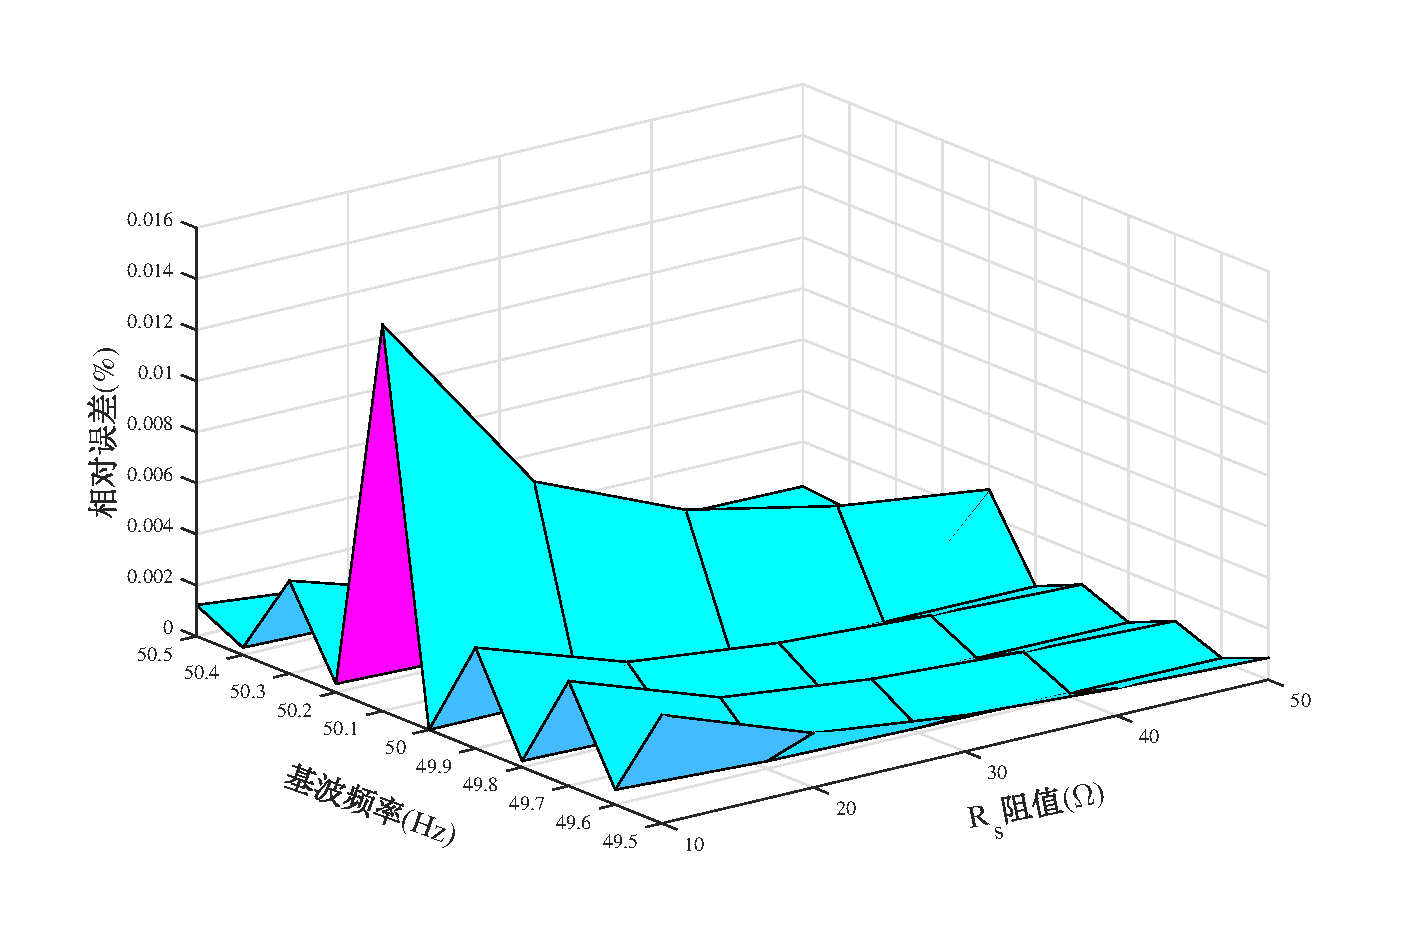
\includegraphics[width=0.9\textwidth]{figures/TR_Fb_TSR}
	\end{figure}
	\vspace{-5.5cm}% 定位说明文字位置,-5.5cm代表从图片下一行处向上移动5.5cm
	% 说明文字(两行)从第2帧之后开始显示,具体位置、字号、字体及高亮显示设置            
	\onslide<2->\qquad\qquad\qquad\qquad \liuhao\kai \alert{当基波频率为~50.1~Hz,$R_s$~为~$10~\Omega$~时误差最大,相对误}\\
	\onslide<2->\qquad\qquad\qquad\qquad\qquad\quad \alert{差不大于~$1.5\times 10^{-2}\%$} \\
	% 定位第二段说明文字位置,为第一段文字后向下移动0.5cm
	\vspace{0.5cm}
	% 说明文字(一行)从第3帧之后开始显示,具体位置、字号、字体及高亮显示设置
	\onslide<3->\qquad\qquad\qquad\qquad\qquad\qquad\qquad \liuhao\kai \alert{随着介损角真值增加,测量误差有逐渐减小的趋势} \\
	% 定位图片标题位置,继续向下移动3.3cm
	\vspace{3.3cm}
	% 图片标题,从第1帧之后开始显示
	\onslide<1->\centering \wuhao 不同阻值条件下的介损角测量误差
\end{frame}
%%%%%%%%%% 图片处理第二帧 %%%%%%%%%%
\begin{frame}
	\frametitle{\vskip -1.5ex\hei\quad 双列图片显示}
	\xiaosi\kai\qquad 窗口长度为~$N=64$~时的~Blackman~窗时频特性
	\begin{figure}
		\centering
		\subfigure[\wuhao 时域特性]{
			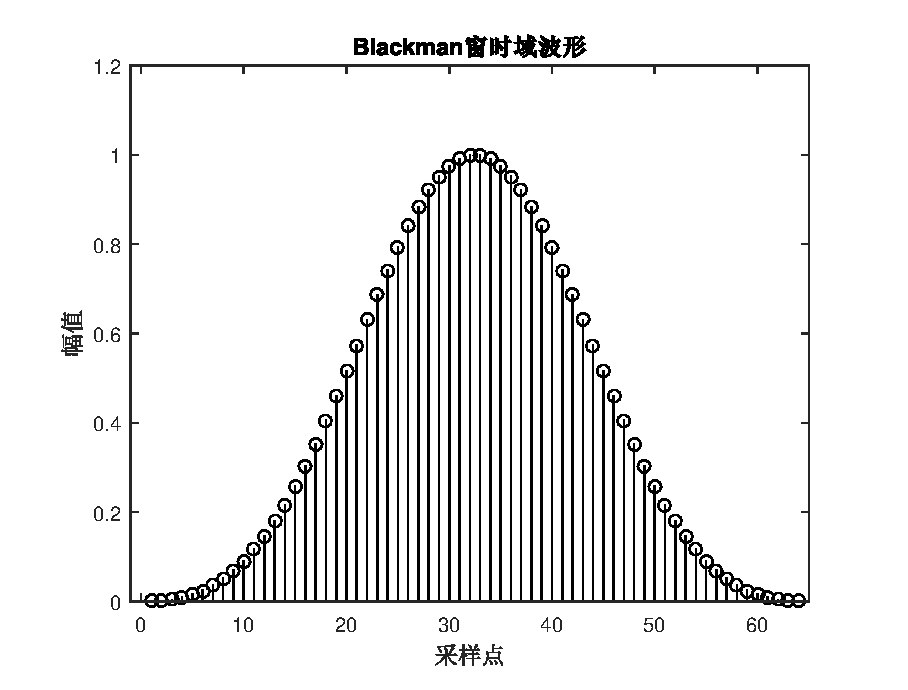
\includegraphics[width=0.45\textwidth]{figures/blackmanTD}}
		\subfigure[\wuhao 幅频特性]{
			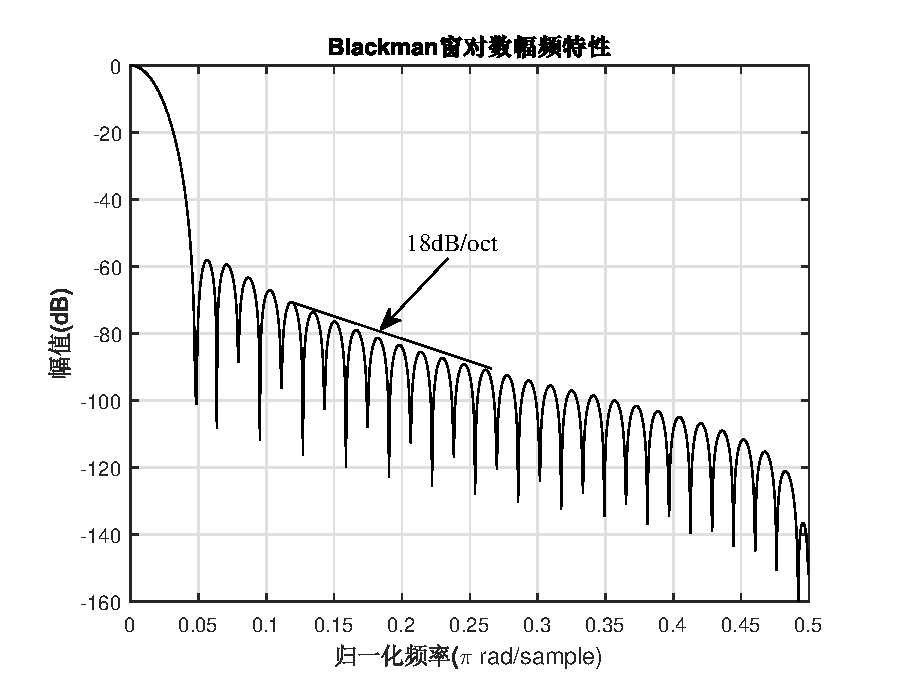
\includegraphics[width=0.45\textwidth]{figures/blackmanAF}}
	\end{figure}
\end{frame}
        % 图片处理
% !Mode:: "TeX:UTF-8"
\section{\sihao\kai\quad {5.~表格处理}}% 章节号及章节名,设置字体字号及对齐
%%%%%%%%%% 表格处理 %%%%%%%%%%
%%%%%%%%%% 表格处理第一帧 %%%%%%%%%%
\begin{frame}
	\frametitle{\vskip -1.5ex\hei\quad 数据表格}
	\begin{table}[htbp]
		\caption{基波频率变化时不同算法频率测量相对误差}
		\centering\kai
		%\rowcolors{2}{tableDeep}{white}
		\begin{tabular}{ccccc}
			\toprule[1.5pt]
			%\rowcolor{tableHead}\bz 频率(Hz) & \bz FFT(\%)      & \bz 算法1(\%) & \bz 算法2(\%) & \bz 算法3(\%)   \\
			                        频率(Hz)   &  FFT(\%)        &   算法1(\%)    &   算法2(\%)    &   算法3(\%)   \\
			\midrule[1pt]
			49.5                              & 2.56E+02         & 0.0108        & 0.0091        & \textbf{0.0006} \\
			49.6                              & 2.02E+02         & 0.0077        & 0.0052        & 0.0004          \\
			49.7                              & 1.49E+02         & 0.0051        & 0.0024        & 0.0003          \\
			49.8                              & 9.73E+01         & 0.0032        & 0.0024        & 0.0002          \\
			49.9                              & 4.74E+01         & 0.0017        & 0.0001        & 9.56E-05        \\
			50.0                              & \alert{1.35E-11} & 0.0007        & 3.4123        & 4.01E-05        \\
			50.1                              & 4.45E+01         & 0.7590        & 3.2765        & 0.0578          \\
			50.2                              & 8.55E+01         & 0.7224        & 3.1330        & 0.0553          \\
			50.3                              & 1.23E+02         & 0.6845        & 2.9825        & 0.0527          \\
			\bottomrule[1.5pt]
		\end{tabular}
	\end{table}
\end{frame}
%%%%%%%%%% 表格处理第二帧 %%%%%%%%%%
\begin{frame}
\frametitle{\vskip -1.5ex\hei\quad 数据表格}
\begin{table}[htbp]
	\renewcommand\arraystretch{1.25}% 是表格里的内容可以看起来居中
	%\renewcommand\arraystretch{1.1}
	\caption{基波频率变化时不同算法频率测量相对误差}
	\centering\kai
	% \rowcolors [<commands>]{<row>}{<odd-row color >}{<even-row color >}
	% \rowcolors{1}{blue!20}{blue!10} 表示从第一行开始,奇数行为蓝色20%,偶数行为蓝色10%。
	\rowcolors{2}{tableDeep}{white}
	\begin{tabular}{ccccc}
		\rowcolor{tableHead}\bz  频率(Hz)  & \bz FFT(\%)     & \bz 算法1(\%)  & \bz 算法2(\%)  & \bz 算法3(\%)   \\
		49.5                              & 2.56E+02                   & 0.0108           & 0.0091        & \textbf{0.0006}\\
		49.6                              & 2.02E+02         & 0.0077        & 0.0052        & 0.0004          \\
		49.7                              & 1.49E+02         & 0.0051        & 0.0024        & 0.0003          \\
		49.8                              & 9.73E+01         & 0.0032        & 0.0024        & 0.0002          \\
		49.9                              & 4.74E+01         & 0.0017        & 0.0001        & 9.56E-05        \\
		50.0                              & \alert{1.35E-11} & 0.0007        & 3.4123        & 4.01E-05        \\
		50.1                              & 4.45E+01         & 0.7590        & 3.2765        & 0.0578          \\
		50.2                              & 8.55E+01         & 0.7224        & 3.1330        & 0.0553          \\
		50.3                              & 1.23E+02         & 0.6845        & 2.9825        & 0.0527          \\
	\end{tabular}
\end{table}
\end{frame}


         % 表格处理
% !Mode:: "TeX:UTF-8"
\section{\sihao\kai\quad 6.~其他内容}% 章节号及章节名,设置字体字号及对齐
%%%%%%%%%% 其他内容 %%%%%%%%%%
%%%%%%%%%% 其他内容第一帧 %%%%%%%%%%
\begin{frame}
	\frametitle{\vskip -1.5ex\quad\hei  动态演示}
	\kai\sihao
	\onslide<1>{只在第一帧中显示}

	\onslide<2->{第二帧之后的所有帧都显示}

	\onslide<1,3>{第一帧和第三帧中显示}

	计数:\only<1>{1}\only<2>{2}\only<3>{3}\only<4->{4}

	\onslide<5>{数完了}
\end{frame}          % 其他
% !Mode:: "TeX:UTF-8"
\section{\sihao\kai\quad 7.~总结}% 章节号及章节名,设置字体字号及对齐
%%%%%%%%%% 总结 %%%%%%%%%%
%%%%%%%%%% 总结第一帧 %%%%%%%%%%
\begin{frame}
	\frametitle{\vskip -1.5ex\quad\hei  总结}
	\kai\xiaosan 本模板比较简单,后续完善工作仍在继续\dots\dots
\end{frame}     % 总结
% !Mode:: "TeX:UTF-8"
\section{\sihao\kai\quad8.~参考文献}% 设置目录中章节名、字体、字号及对齐
%%%%%%%%%% 参考文献 %%%%%%%%%%
%%%%%%%%%% 参考文献第一帧 %%%%%%%%%%
\begin{frame}%[allowframebreaks]% 允许参考文献多张PPT显示
    \frametitle{\vskip -1.5ex\quad\hei  参考文献}
    \small
    \printbibliography
    % 如果想单独在某页插入参考文献,请注释掉上面的代码,采用如下代码:
    %\begin{thebibliography}{10}
    %\beamertemplatebookbibitems% 显示书的图标,注释掉默认是文章de 图标
    %\small
    %\bibitem{Gantmakher} F. R. Gantmakher, Theory of matrices, Russian, Nauka, Moscow, 1959.
    %\end{thebibliography}
\end{frame}            % 参考文献
%%%%%%%%%% 演示文稿结束页背景 %%%%%%%%%%
\usebackgroundtemplate{% 此处设置结束页页背景图片
	
\includegraphics[width=\paperwidth,height=\paperheight]{img/end.png}
}
%%%%%%%%%% 演示文稿结束页内容 %%%%%%%%%%
\begin{frame}
	\centering
	\Huge\kai\textcolor{hnuBlue}{谢谢各位老师与同学!\\
		\vskip 0.1cm
		敬请指导!}
\end{frame}
\end{document}
